\newpage
\section{Технологическая часть}

\subsection{Руководство по интеграции и настройке подсистемы}
Одной из целей при создании ПОАПО являлось создание удобного и простого в интеграции с другими системами модуля для автономной навигации объектов. Руководствуюясь этой целью, процесс установки и настройки был максимально упрощен. 
Для корректной работы подсистемы необходимо использовать оборудование, указанное в техническом задании к системе, а именно:
\begin{itemize}
\item требования к цифровой камере:
	\begin{itemize}
	\item разрешение не ниже 1 Мп;
	\item интерфейс соединения со скоростью не ниже 12 Мбит/с;
	\item жесткое крепление на объекте;
	\end{itemize}
\item Требования к инерциальному измерительному устройству 
 	\begin{itemize}
 	\item трехосевой гироскоп с диапазоном измерения до 2000 $^\circ$/с и точностью не ниже, чем 0,2$^\circ$ на 1 $^\circ$/с;
	\item акселерометр с тремя степенями свободы и дипазоном измерения $\pm10g$.
 	\end{itemize}
\end{itemize}

Вторым этапом интеграции является жесткое закрепление камеры и ИИУ на подвижном объекте, перемещения которого и предполагается расчитывать. Камеру необходимо расположить по направлению движения и так, чтобы в кадре 70\% изображения занимала горизонтальная поверхность, по которой происходит движение, и 30\% кадра занимали объекты, расположенные над линией горизонта.  

Далее нужно провести каллибровку камеры для выявления внутренних и внешних параметров камеры. С теоретической точки зрения данных процесс описан в пункте~\ref{part:calibrateCamera}. На практике процесс является более простым и заключается в виксации <<специального изображения>> камерой и последующем анализе полученного изображения. Данный метод калибровки называется <<новым гибким методом калибровки камеры>> и был предложен Zhengyou Zhang\cite{Zhang}. Как правило в качестве <<специального изображения>> используется изображения шахмотной доски. Суть методоа заключается в нахождении углов такой доски и подбору внутренних параметров камеры таким образом, чтобы на изображении эти углы выстраивались в прямые линии. Для корректного опредления параметров камеры желательно получить как можно больше изображений такой доски под разными углами. Схематично данный процесс отображен на рисунке~\ref{pic:calibrationMan}.

\begin{figure}[!h]
\center{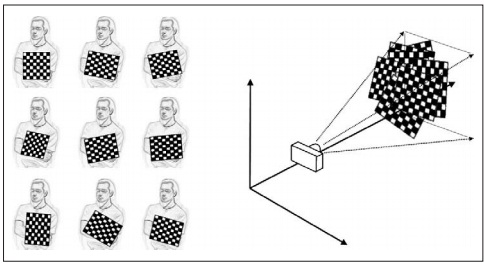
\includegraphics[width=0.8\linewidth]{pics/calibrationMan.png}}
\caption{Процесс гибкого метода калбровка камеры.}
\label{pic:calibrationMan}
\end{figure}

В то же время, данный метод можно применять для вычисления матрицы трасформации изображений. Рассмотрим рисунок~\ref{pic:perspectiveTranform}. Если фиксирвоать изображения шахматной доски в плоскости левой фигуры, то при удалении искажений мы получим изображение строго перпендикулярное камере. В визуальной одометрии наоборот необходимо отобразить все клюевые точки в плоскости пола. Таким образом, получив матрицу изменения изображения, транспанируем ее и будем применять для нормализованных изображений с целью опрделить реальное положение ключевых точек кадра на плоскости перемещения. 

\begin{figure}[!h]
\center{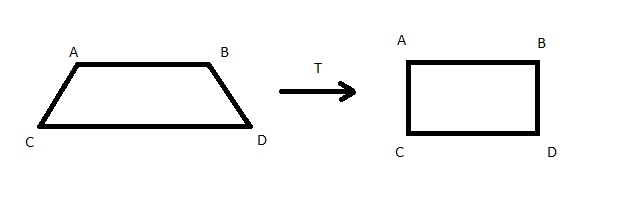
\includegraphics[width=0.8\linewidth]{pics/perspectiveTransform.png}}
\caption{Принцип перспективного преобразования изображений.}
\label{pic:perspectiveTranform}
\end{figure}

После устновки необходимого оборудования и его калибровки необходимо согласовать программный интерфейс подсистемы для корректного передачи видеоряда и данных с ИИУ. 
Подсистема ПАОПО предоставляет следующий API:

PutNewData


\subsection{Диаргамма взаимодейсвия компонентов}
В ходе работы подсистемы происходит взаимодейсвие ее модулей между собой и с внешними системами. Диаграмма последовательности такого взаимодейсвия показна на рисунке~\ref{pic:secquence}.

\afterpage{
\clearpage
%\thispagestyle{empty}
\begin{landscape}
\begin{center}
	\begin{figure}[H]
	\center{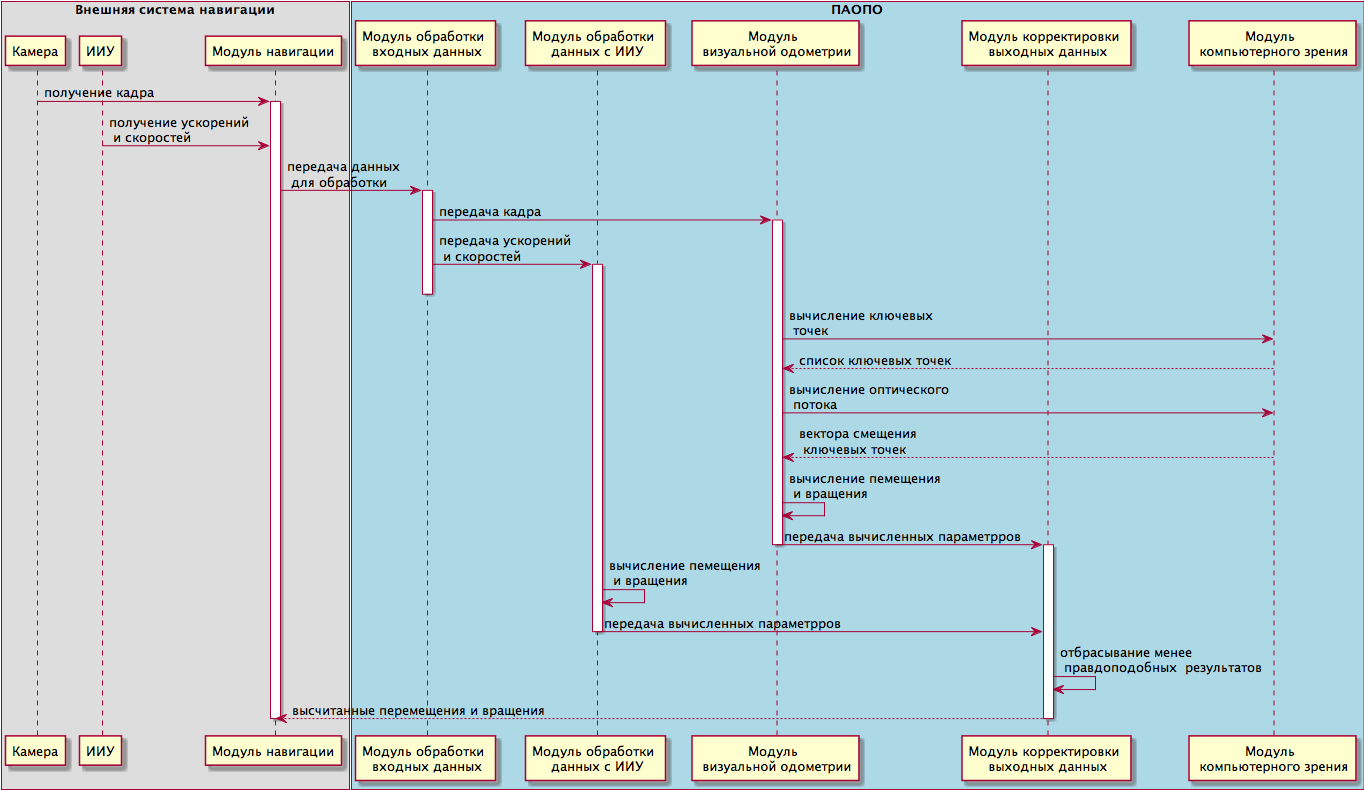
\includegraphics[width=1\linewidth]{pics/sec.png}}
	\caption{Диаграмма последовательности взаимодейсвия компонентов.}
	\label{pic:secquence}
	\end{figure}
\end{center}
\end{landscape}
\clearpage
}


\subsection{Диаграмма классов подсистемы}
При реализации прототипа рассматриваемой подсистемы был написан программный продукт на  языке Java в программном пакете JetBrains IDEA. В качестве модуля компьютерного зрения использовалась библиотека OpenCV (Open Computer Vision). 
В результате был получен программный продукт состоящий из нескольких классов, связанных между собой. Получившаяся диаграмма классов представлена на рисунке~\ref{pic:classDiagram}.


\begin{figure}[!htb]
\center{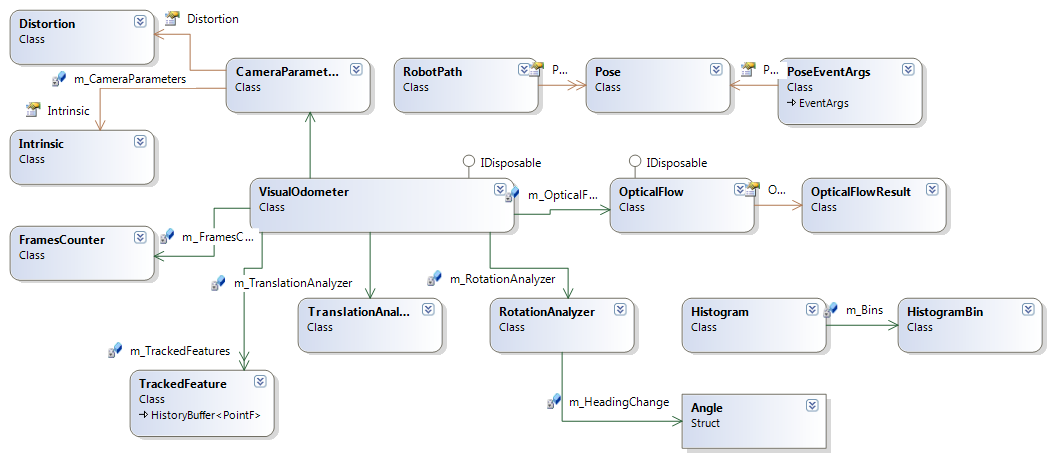
\includegraphics[width=0.9\linewidth]{pics/classDiagram.png}}
\caption{Диаграмма классов прототипа подсистемы.}
\label{pic:classDiagram}
\end{figure}